\chapter{Objectifs}

Le but de ce projet est de fournir une solution permettant de protéger les applications
du client sur Windows en évitant leur copie ou leur utilisation illégale. 
Il devra également permettre au client de générer et gérer des licences d'utilisations 
via une interface graphique. Il pourra ainsi définir des contraintes sur les licences 
comme par exemple leur durée de validité. \newline

Cet outil vient en remplacement de solutions déjà existantes telles que IntellilLock ou ElecKey,
à l'instar de ces outils la prise en compte des paiements sera effectuée par une solution externe
du client.

\chapter{Terminologies}

\begin{itemize}
	\item Le client est le commanditaire du projet.
	\item Un utilisateur est une personne souhaitant utiliser un logiciel du client. 
	\item Une licence est un droit accordé pour une machine et un utilisateur d'utiliser un logiciel donné.
\end{itemize}

\chapter{Exigences fonctionnelles}

\section{Plateforme d'enregistrement}
Nous devrons fournir une platefrome d'enregistrement pour les utilisateurs, avec une interface simple, facile d'accès et lisible notamment pour des personnes sans compétences en informatiques. Il faudra donc que l'outil dispose :
\begin{itemize}
	\item Un guide du site avec un tutoriel pour s'enregistrer et créer une licence.
	\item Une page de contact pour demander de l'aide.
	\item Une charte graphique épurée en suivant les recommandations matérial design.
\end{itemize}
Cette plateforme sera également utilisé par la suite pour effectuer la demande d'une licence pour un logiciel au client.

\section{Vérification d'une licence}
Un programme devra permettre de vérifier la validité et l'authenticité d'une licence pour un logiciel. Les attributs à considérer lors de la vérification sont les suivants :
\begin{itemize}
    \item La date de validité.
    \item Le nombre d'essais.
\end{itemize}

Dans un premier temps, le programme devra être intégré par le client lors du developpement de son application puis, dans un second temps, il pourra être directement ajouté au logiciel sans avoir besoin de modifier le code source.

\section{Plateforme administrateur}
Cette platefrome devra permettre au client de donner les autorisations nécessaires à un profil d'un utilisateur afin que celui-ci puisse par la suite générer une licence.
Pour cela il pourra accéder à un panneau de contrôle avec les options suivantes:

\begin{itemize}
	\item La liste des profils utilisateurs.
	\item Une liste des nouveaux utilisateurs en attente de validation.
	\item La possibilité de consulter les licences de chaque utilisateur.
	\item La possibilité de définir la portée d'une licence pour un utilisateur comme la durée de validité (potentiellement infinie) ou des restrictions.
\end{itemize}
\newpage

\chapter{Exigences techniques}

\section{Exigences de sécurité}
Les principaux points liés aux aspects de la sécurité sont les suivants:
\begin{itemize}
	\item Entraver les tentatives de reverse engineering via l'obfuscation du code de l'application (cf. Fiches Techniques - Obfuscation de code).
	\item Les échanges de données sur le réseau seront chiffrés.
	\item Le stockage des données persistantes sera lui aussi protégé (cf. Fiches techniques - Sécurisations des bases de données).
\end{itemize}

\section{Exigences opérationnelles}

L'outil développé dans le cadre de ce projet devra être utilisable sous Windows, et aura pour but de protéger des logiciels conçus pour Windows également.

Il devra être compatible avec les dernières versions de Windows (Windows 8, 10 et 11).

\section{Exigences de qualité}

Tout au long du développement ce projet, nous devront nous assurer d'une certaine exigence de qualité.

Il faut que le code soit réutilisable, maintenable et facilement compréhensible donc correctement documenté.
Il nous faudra suivre (voir définir) une certaine charte de code permettant un formalisme, et donc une homogénéité dans
le code source du projet. Ce dans le but de pouvoir confier ce projet à une autre équipe qui pourra le reprendre et le developper.

Il faudra aussi s'assurer de la qualité de l'expérience utilisateur et administrateur.
Les utilisateurs ne seront pas familiés au domaine de l'informatique, il faudra penser les 
interfaces les plus intuitives possible. De même pour les outils administrateurs dont la gestion devra 
être facile, le client ayant de nombreuses licences à gérer. 

\chapter{Spécifications fonctionnelles de l'outil}

\section{Partie utilisateur}

Cette section décrit comment l'utilisateur pourra intéragir avec notre outil. Cette interaction est décrite dans le schéma n°\ref{fig:fig1}.
\newline

\begin{itemize}
	\item \textbf{Inscription d'un utilisateur} \newline
	Un utilisateur pourra s'inscrire via une interface afin de pouvoir obtenir une licence qui lui permettra d'utiliser le logiciel souhaité. (étape I)
	Sur cette même interface il pourra choisir le logiciel dont il souhaite obtenir une licence et en effectuer la demande.
	\item \textbf{Génération de la licence} \newline
	Une fois inscrit, si le client a validé la demande de licence (voir 5.2.1), l'utilisateur devra télécharger un outil, depuis la plateforme, afin de générer la licence. (étape III)
	\item \textbf{Utilisation du logiciel avec la licence} \newline
	La licence obtenue, l'utilisateur pourra alors débloquer le logiciel protégé qu'il souhaite utiliser en lui renseignant sa licence. (étape IV)
\end{itemize}

\section{Partie client}

\begin{itemize}
	\item \textbf{Activation d'un compte et gestion des droits} \newline
	Lorsque qu'un utilisateur se créera un compte et effectuera une demande de licence, notre client pourra, ou non, 
	répondre à sa demande et lancer la génération de licence via son interface administrateur (étape II)
	\newline
	La partie paiement du logiciel ne sera pas pris en charge par notre outil, à la demande du client,
	il devra effectuer lui-même les vérifications.
\end{itemize}

\newpage

\begin{figure}[h]
	\centering
	\vspace{4cm}
	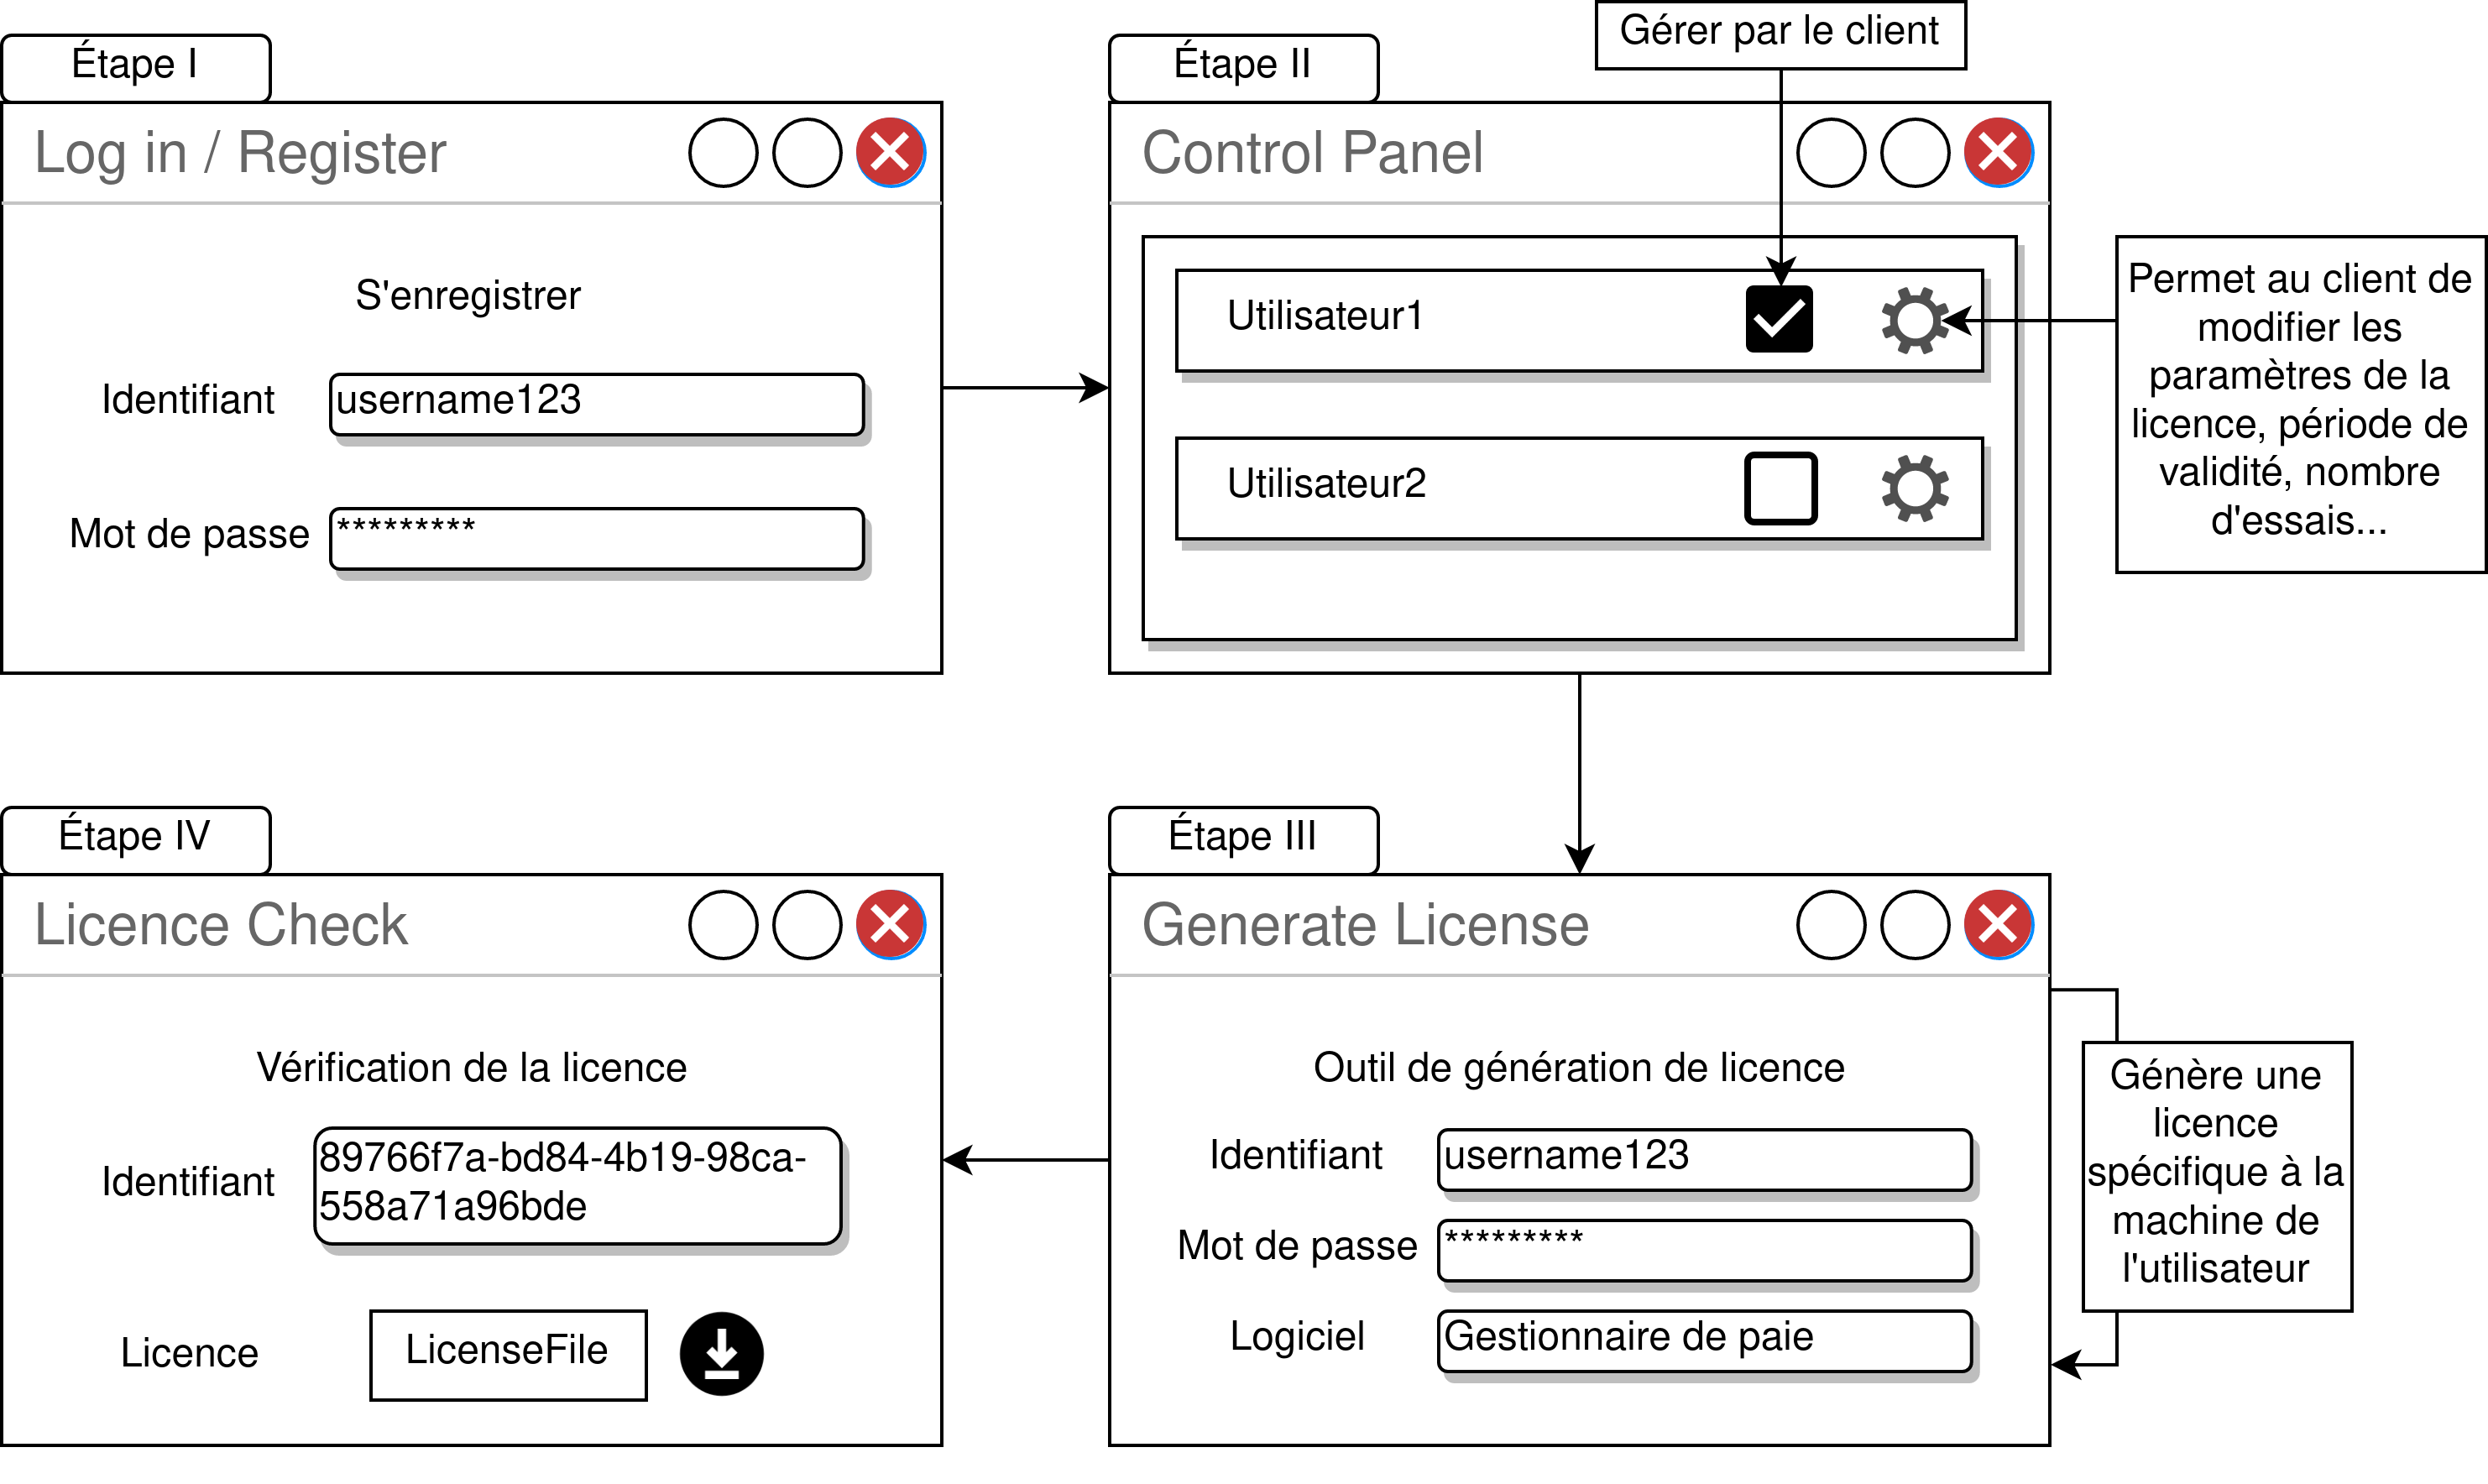
\includegraphics[width=18cm]{main/png/STB.png}
	\caption{Schéma décrivant le fonctionnement général de la solution}
	\label{fig:fig1}
\end{figure}

\newpage

\section{Diagramme des cas d'utilisations}

\begin{figure}[h]
	\centering
	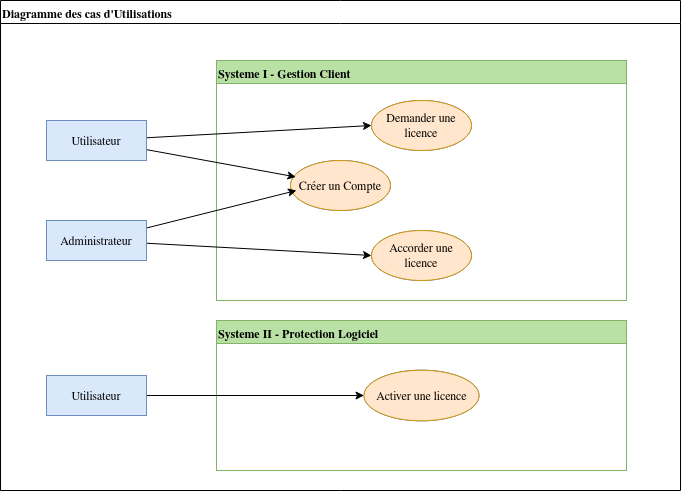
\includegraphics[width=16cm]{main/png/Util.png}
	\caption{Diagramme des cas d'utilisations}
	\label{fig:fig2}
\end{figure}

\section{Tableau des cas d'utilisations}

\begin{table}[h]
	\centering
	\begin{tabular}{ | m{0.6cm} | m{6cm} | m{6cm}| m{3cm} | } 
                \hline
		\textbf{ID} & \textbf{Intitulé} & \textbf{Acteurs} & \textbf{Priorité} \\
                \hline
			1 & Demande de licence & Utilisateur & Indispensable \\
                \hline
			2 & Accord de licence & Administrateur & Indispensable \\
                \hline
			3 & Activation d'une licence & Utilisateur & Indispensable \\
		\hline
			4 & Création d'un compte & Utilisateur et administrateur & Important \\
		\hline
			5 & Paramétrage d'une licence & Administrateur & Important \\
		\hline
        \end{tabular}
	\caption{Tableau des cas d'utilisations}
	\label{tab:tab1}
\end{table}
\newpage

\section{Cas d'utilisations}

\subsection{Cas d'utilisation 1 et 2 : Demande et accord de licence}

\begin{table}[!h]
	\centering
	\begin{tabular}{| m{4cm} | m{12cm} |}
		\hline
		    \textbf{Acteurs concernés} & Un utilisateur et un administrateur. \\
		\hline
		    \textbf{Description} & Un utilisateur effectue, via la plateforme, une demande pour obtenir une licence pour un logiciel souhaité. Cela provoque une notification pour l'administrateur, qui peut ensuite accorder ou non à l'utilisateur la licence, via la plateforme également, selon qu'il ait reçu ou non le paiement. \\
		\hline
		    \textbf{Pré-conditions} & L'utilisateur doit s'être enregistré sur la plateforme.\\
		\hline
		    \multicolumn{2}{|c|}{\textbf{Schéma de séquence :}} \\
		\hline
		    \multicolumn{2}{|c|}{}\\
		    \multicolumn{2}{|c|}{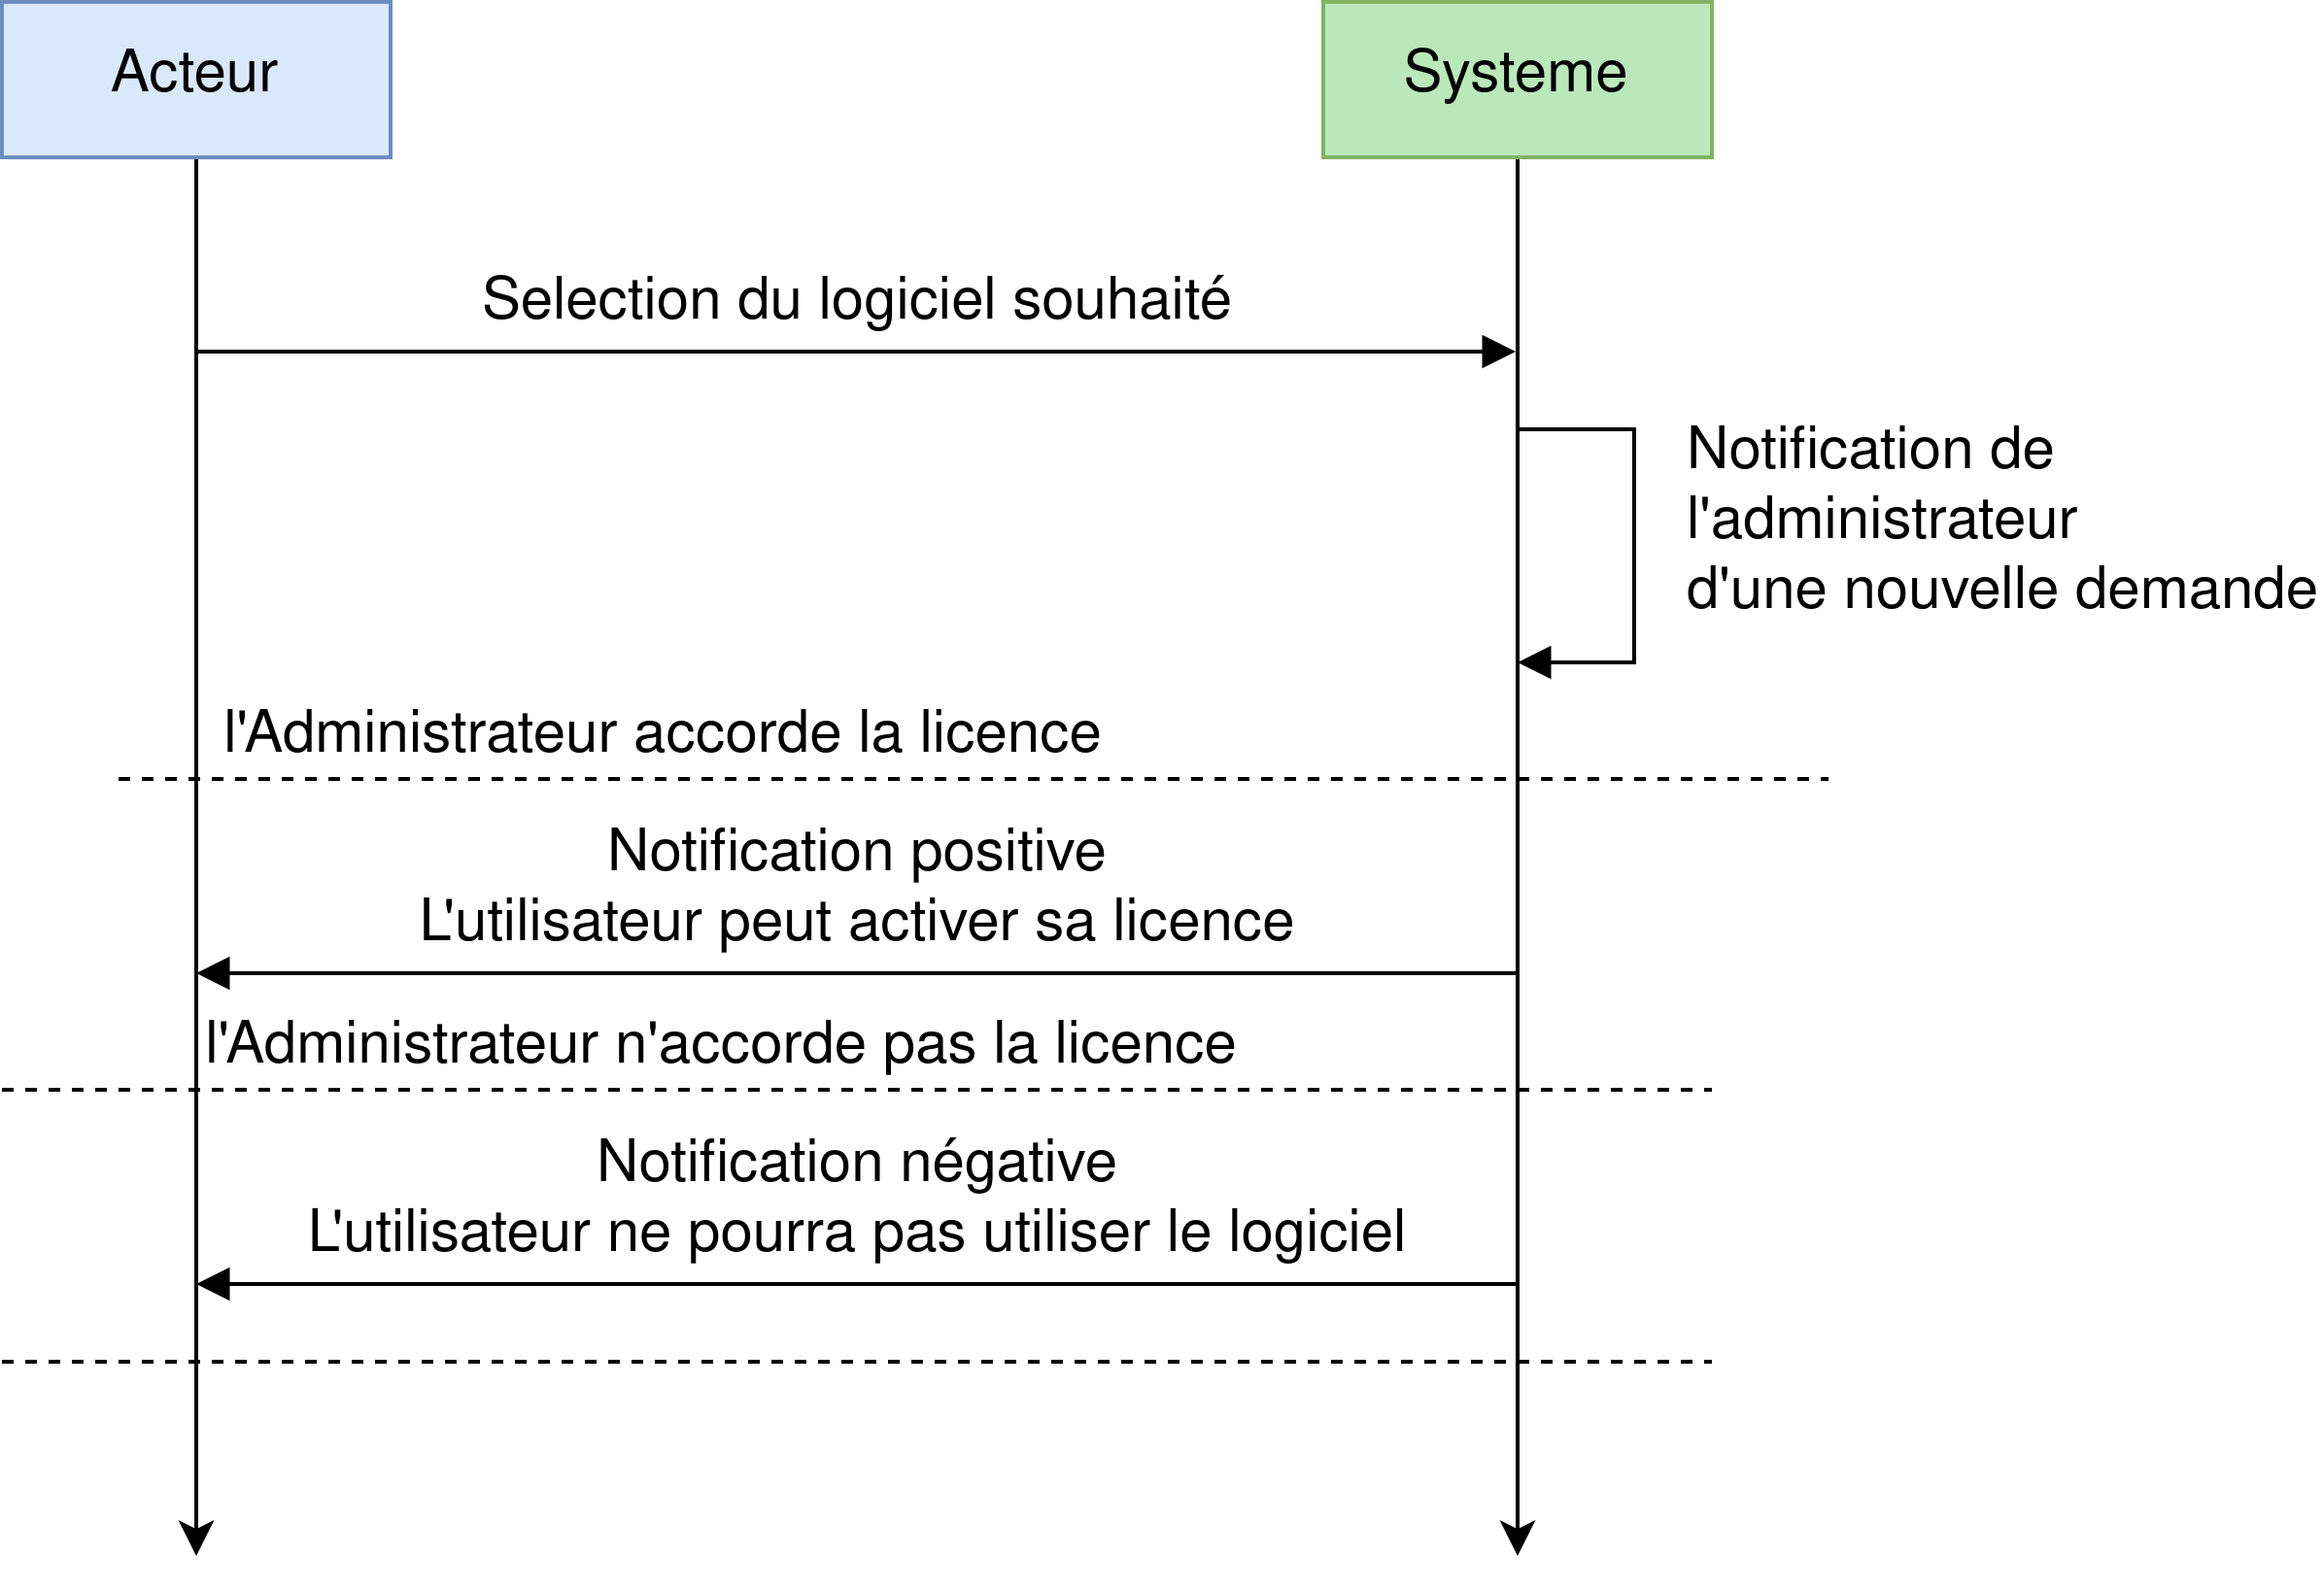
\includegraphics[width=15cm]{main/png/seq_demande.png}} \\
		\hline
	\end{tabular}
	\label{tab:tab2}
\end{table}
\newpage

\subsection{Cas d'utilisation 3 : Activation d'une licence}

\begin{table}[!h]
        \centering
        \begin{tabular}{| m{4cm} | m{12cm} |}
                \hline
		    \textbf{Acteurs concernés} & Utilisateur. \\
                \hline
		    \textbf{Description} & L'utilisateur souhaite activer le logiciel du client après avoir obtenu une licence. Pour ce faire il télécharge le logiciel d'activation sur la plateforme, puis s'y connecte afin de pouvoir récupérer les licences souhaitées.\newline
		    L'utilisateur devra procéder de la même manière dans le cas d'une extension ou d'une autre modification de sa licence.\\
                \hline
		    \textbf{Pré-conditions} & L'utilisateur est enregistré sur la plateforme, et pour récupérer ses licences elles doivent avoir été accordées par l'administrateur.\\
		\hline
		    \multicolumn{2}{|c|}{\textbf{Schéma de séquence :}} \\
                \hline
                    \multicolumn{2}{|c|}{}\\
                    \multicolumn{2}{|c|}{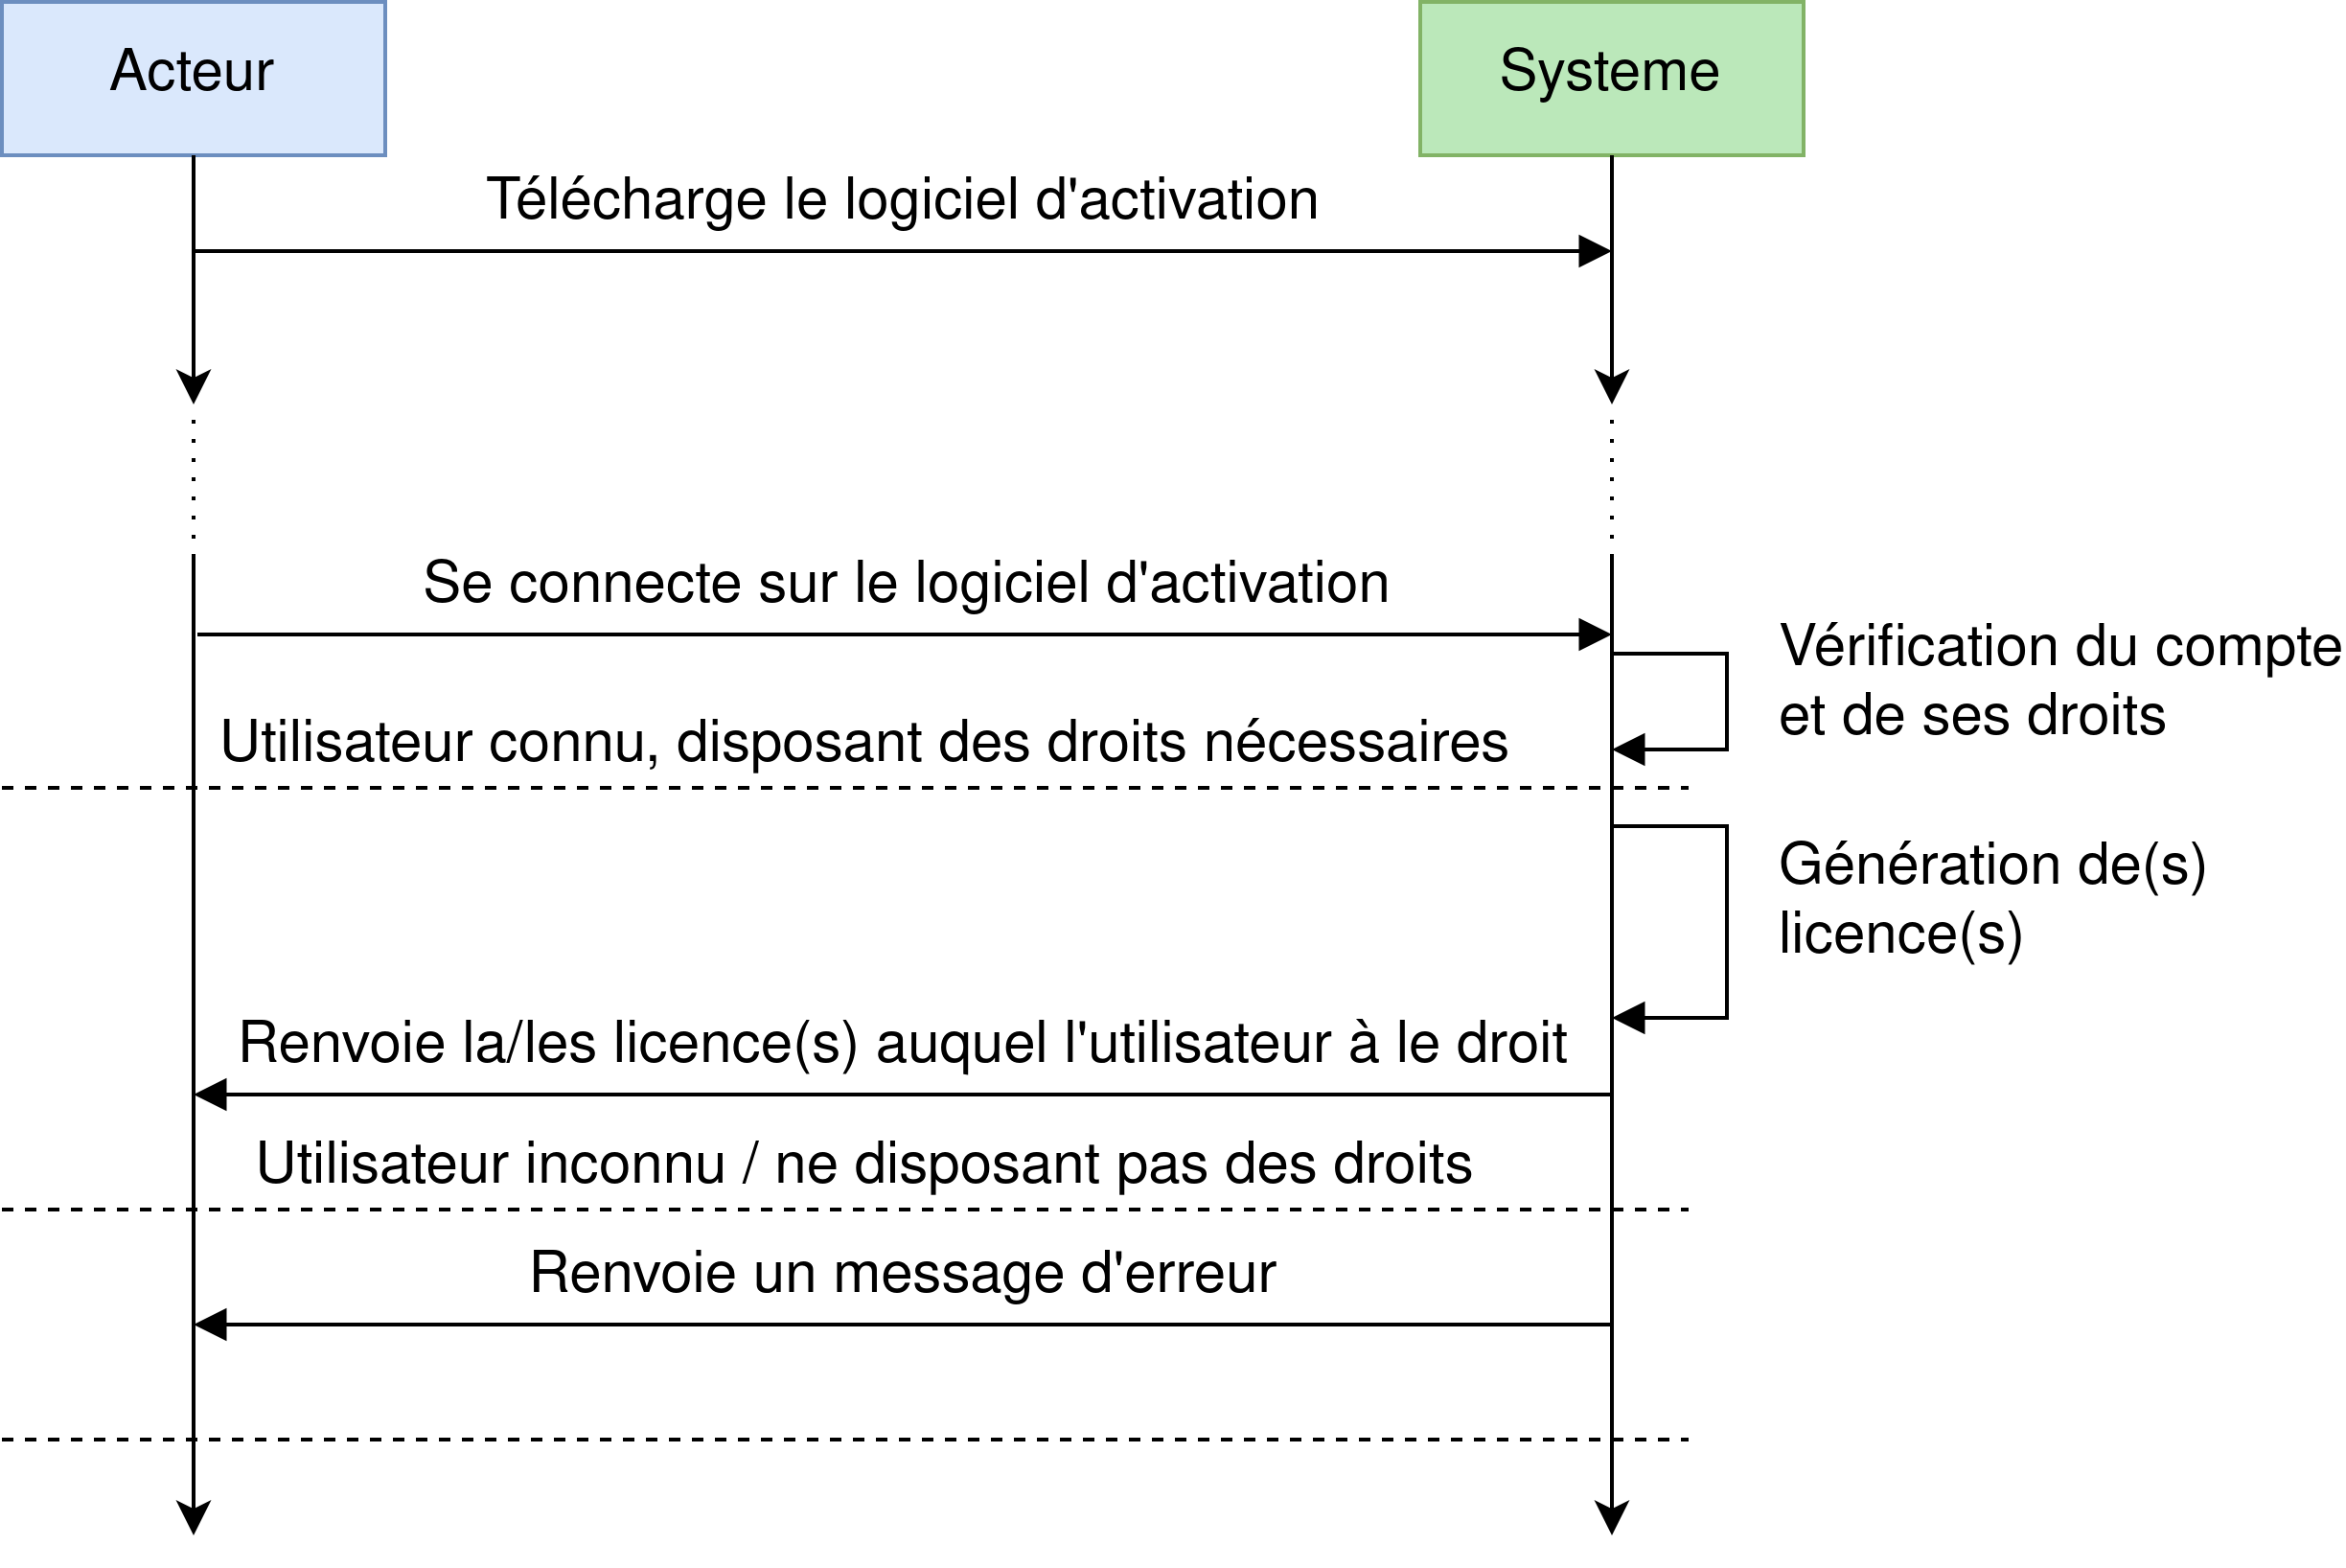
\includegraphics[width=15cm]{main/png/seq_activation.png}} \\
                \hline
        \end{tabular}
        \label{tab:tab3}
\end{table}
\newpage

\subsection{Cas d'utilisation 4 : Création d'un compte}

\begin{table}[!h]
        \centering
        \begin{tabular}{| m{4cm} | m{12cm} |}
                \hline
		    \textbf{Acteurs concernés} & Utilisateur. \\
                \hline
		    \textbf{Description} & Un utilisateur souhaite créer un compte sur notre plateforme dans le but d'obtenir une licence. \\
                \hline
		    \textbf{Pré-conditions} & L'identifiant et le mot de passe de l'utilisateur doivent respecter certaines conditions (voir \textbf{RG\#2.1}).\\
		\hline
		    \multicolumn{2}{|c|}{\textbf{Schéma de séquence :}} \\
                \hline
                    \multicolumn{2}{|c|}{}\\
                    \multicolumn{2}{|c|}{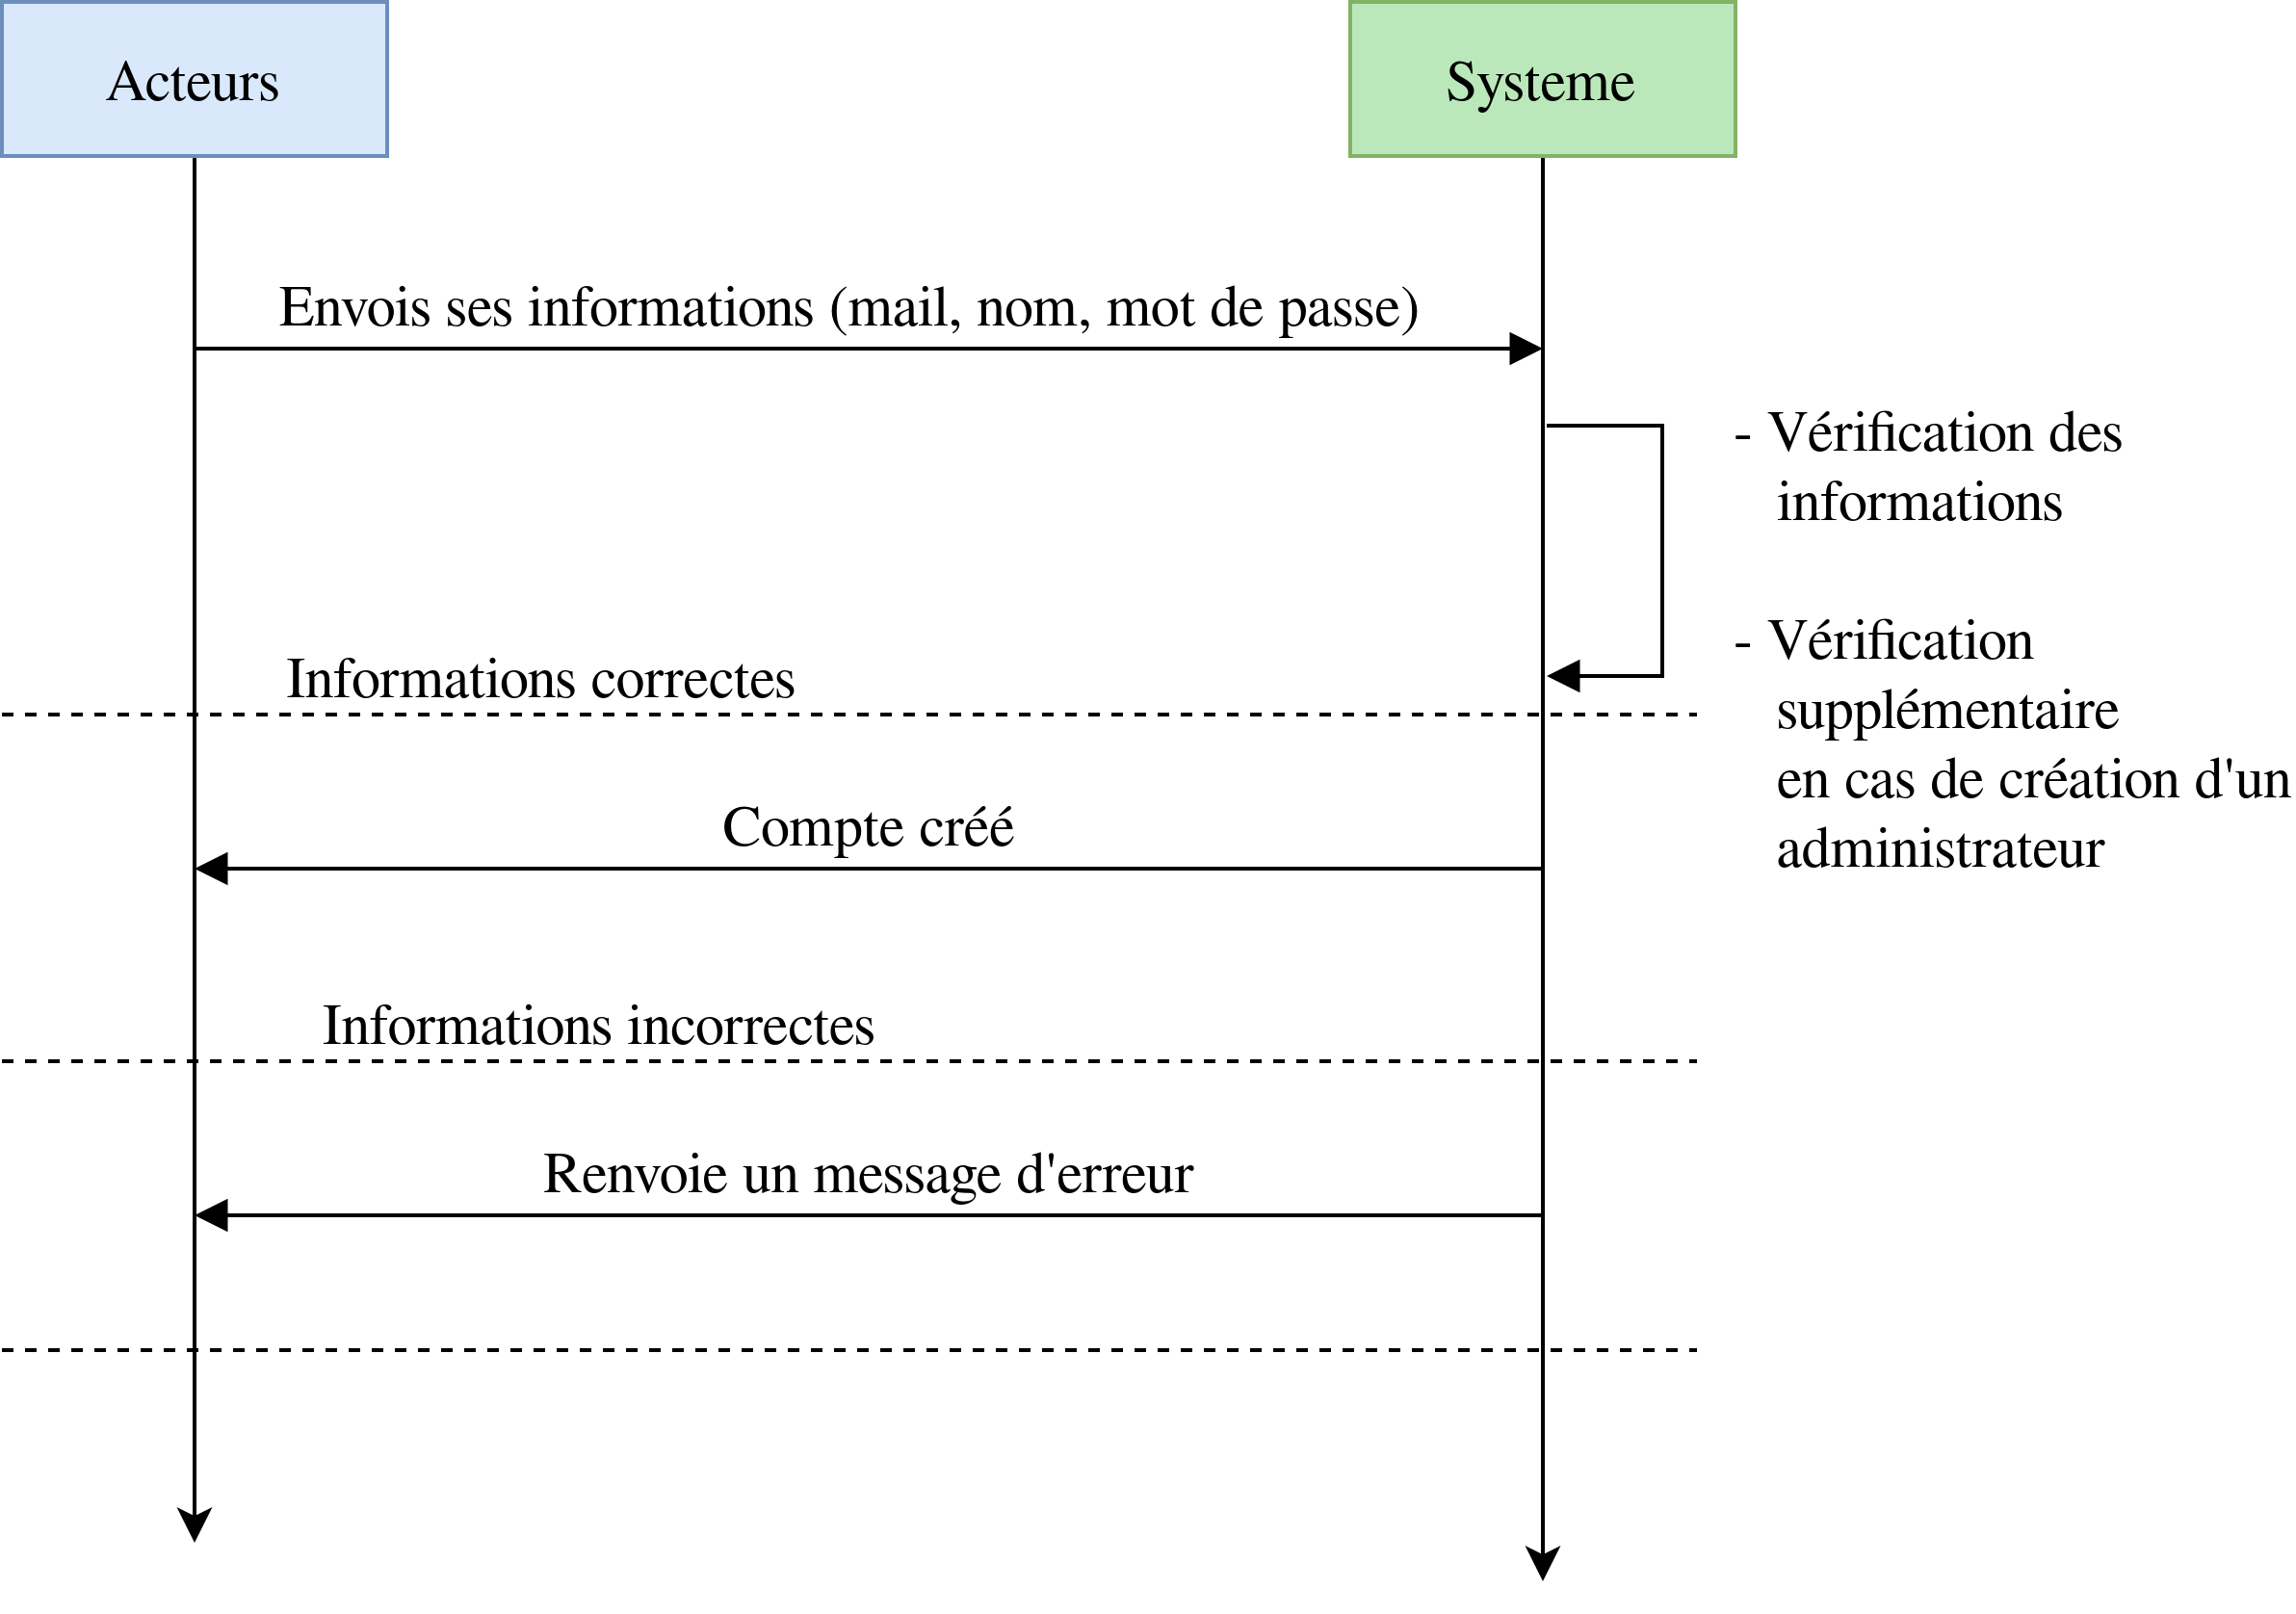
\includegraphics[width=15cm]{main/png/seq_creation.png}} \\
                \hline
        \end{tabular}
        \label{tab:tab4}
\end{table}
\newpage

\subsection{Cas d'utilisation 5 : Paramétage d'une licence}

\begin{table}[!h]
        \centering
        \begin{tabular}{| m{4cm} | m{12cm} |}
                \hline
		    \textbf{Acteurs concernés} & Administrateur. \\
                \hline
		    \textbf{Description} & Un administrateur souhaite modifier les paramètres de la licence d'un des ces client, par exemple étendre la validité d'une licence d'un an. Pour cela il se connecte sur la plateforme et peut modifier cela sur le profil de l'utilisateur. L'utilisateur est ensuite notifié de ces changements afin d'actualiser sa licence.\\
                \hline
		    \textbf{Pré-conditions} & L'utilisateur possède déjà une licence.\\
		\hline
		    \multicolumn{2}{|c|}{\textbf{Schéma de séquence :}} \\
                \hline
                    \multicolumn{2}{|c|}{}\\
                    \multicolumn{2}{|c|}{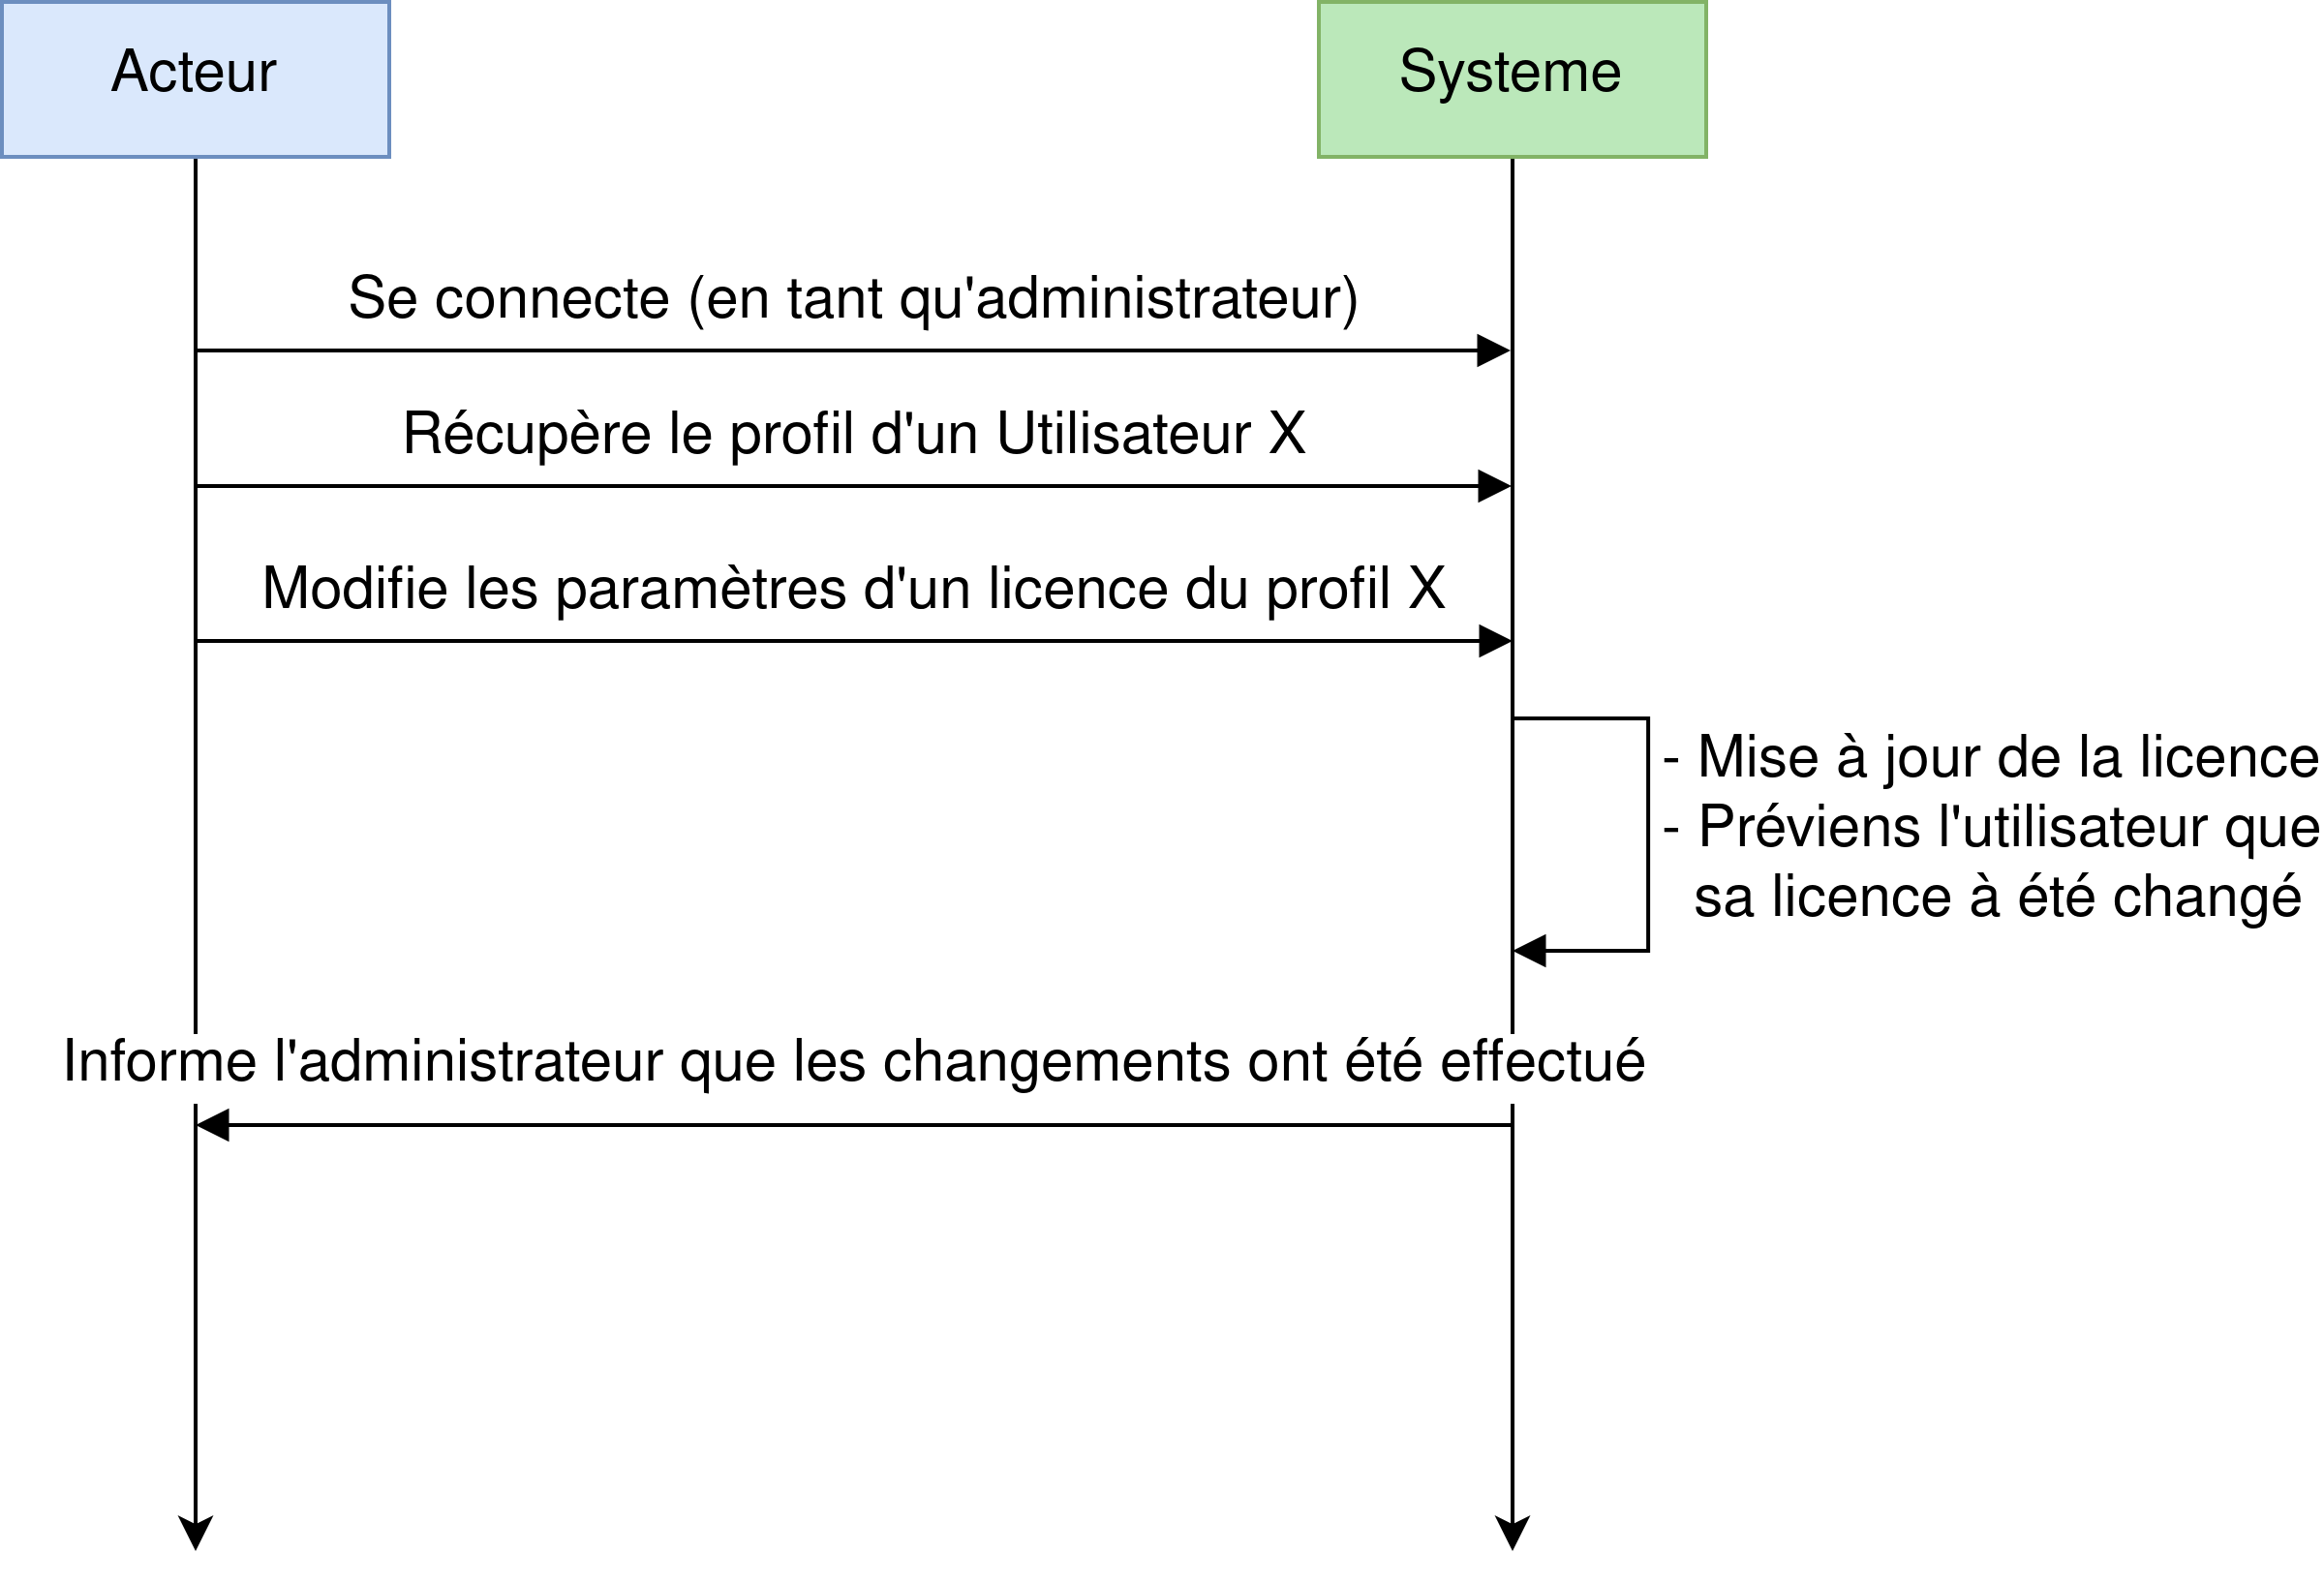
\includegraphics[width=15cm]{main/png/seq_parametrage.png}} \\
                \hline
        \end{tabular}
        \label{tab:tab5}
\end{table}
\newpage

\section{Règles de gestion}

\subsection{Demande d'une licence}
	
\begin{table}[!h] % <-- Super important in order to anchor at the top of the document
    \small
    \begin{tabular}{|m{1.5cm}|m{1.9cm}|m{2.5cm}|m{2.5cm}|m{7cm}|}
	\hline
	    \textbf{ID} & \textbf{Action} & \textbf{Entrée} & \textbf{Sortie} & \textbf{Description} \\
	\hline
	    \textbf{RG\#1.1} & Demande de licence & Logiciel sélectionné & Message de confirmation  d'envoi & Notification à l'administrateur après réception de la demande dans la table correspondante de la base de données \\
	\hline
	    \textbf{RG\#1.2} & Réception d'une  demande de  licence & Identifiant utilisateur \& logiciel & Notification informative à l'utilisateur  confirmant ou  non la demande  précédente & Envoi d'une notification sur la plateforme à l'utilisateur quant à sa demande et ajout de la nouvelle demande à la base de données\\
	\hline
    \end{tabular}
\end{table} 
	
\subsection{Création d'un compte utilisateur/administrateur}

\begin{table}[!h] % <-- Super important in order to anchor at the top of the document
    \small
    \begin{tabular}{|m{1.5cm}|m{1.9cm}|m{2.5cm}|m{2.5cm}|m{7cm}|} 
	\hline
	    \textbf{ID} & \textbf{Action} & \textbf{Entrée} & \textbf{Sortie} & \textbf{Description} \\
	\hline
	    \textbf{RG\#2.1} & Création de compte sur la  plateforme & Mot de passe (contenant au moins 6 caractères et un spécial) et mail valides & Message informatif de création de compte, accès à la plateforme de demande de licence& Ajout à la table de comptes de la base de données et notification à l'administrateur après l'ajout à la base de données en cas de validation de la vérification\\
	\hline
	    \textbf{RG\#2.2} & Vérification des informations de  compte renseignées & Mot de passe et mail renseignés précédement & Retour de test des mots de passe et mail renseignés pour la création de compte& Notification à la création de compte en cas de succès de la vérification ce qui permet l'ajout à la table des comptes et l'envoie d'une notification de création de compte valide à l'utilisateur ainsi qu'a l'administrateur\\
	\hline
    \end{tabular}
\end{table}

\newpage
\subsection{Paramétrage d'une licence}

\begin{table}[!h] % <-- Super important in order to anchor at the top of the document
    \small
    \begin{tabular}{|m{1.5cm}|m{1.9cm}|m{2.5cm}|m{2.5cm}|m{7cm}|} 
	\hline
	    \textbf{ID} & \textbf{Action} & \textbf{Entrée} & \textbf{Sortie} & \textbf{Description} \\
	\hline
	    \textbf{RG\#3.1} & Connexion au gestionnaire de licence & Identifiant \& Mot de passe administrateur & Plateforme de gestion  des demande de licences utilisateurs & La plateforme permet un paramétrage et des modifications des licences en fonction des licences accordées à l'utilisateur contenu dans la base de données\\
	\hline
	    \textbf{RG\#3.2} & Paramétrage  des licences& Identifiants utilisateur \&  logiciel demandé & Notification utilisateur après le paramétrage de la licence par l'administrateur & Notification et message informatif pour l'utilisateur et l'administrateur quant aux modifications apportées après la mise à jour de la base de données grâce au paramétrage\\
	\hline	    
    \end{tabular}
\end{table}

\subsection{Activation d'une licence}

\begin{table}[!h] % <-- Super important in order to anchor at the top of the document
    \small
    \begin{tabular}{|m{1.5cm}|m{1.9cm}|m{2.5cm}|m{2.5cm}|m{7cm}|} 
	\hline
	    \textbf{ID} & \textbf{Action} & \textbf{Entrée} & \textbf{Sortie} & \textbf{Description} \\
	\hline
	    \textbf{RG\#4.1} & Gestion des licences sur la plateforme & Sélection du logiciel pour l'activation & Notification à l'utilisateur du téléchargement du logiciel d'activation de sa licence & Vérification dans sa base de donnée si il y a correspondance aux licences. Si oui, alors le logiciel renvoie les licences cours de validité de l'utilisateur, pour pouvoir accéder aux logiciels \\ 
	\hline
	    \textbf{RG\#4.2} & Connexion sur  le logiciel  d'activation &  Mot de passe et mail administrateur dans la base de données des comptes & Accés pour l'utilisateur à sa platefrome de gestion de ses licences et à leurs logiciels d'activation & Vérification dans sa base de donnée si il y a correspondance aux entrées données. Si oui, alors active une licence et renvoie les licences en cours de validité. Sinon envoie un message de refus \\ 
	\hline
    \end{tabular}
\end{table}
